\section{Higher-Dimensional Ising Models}

% A few logistical points. Midterm exam is this week, oral + online. Please schedule via email.

\subsection{Attacking the Ising Model in Arbitrary Dimension}
We have been discussing various solvable models - the 1D Ising model, the infinite range model, the spherical model and so on. Each of these had a wonderful trick to find the solution. We found results like the critical exponents for these models. Although we didn't go through the derivation, we also discussed the Ising model, gave a plausibility argument for the solution, and gave the solution. But beyond 2D, there really is not an approach that gives us the exact solution. So, this is the end of the analytically known - but this is not a huge problem as most physical systems are not solvable anyway. So, what we will start to do now is an attack on the higher dimensional Ising models (of which we will take a more systematic approach to later).

We have the Hamiltonian:
\begin{equation}
    H = -J\sum_{x, i}\sigma_x\sigma_{x+i} - \sum_x B_x\sigma_x
\end{equation}
generally we consider $B$ position-independent (and we also will generally set $B$ to zero) but here we make it position dependent temporarily so we can take derivatives of the partition function with respect to it.

So, to make contact with thermodynamics, let us write down the partition function:
\begin{equation}
    Z = \sum_{\text{spins}} e^{-\frac{H}{k_B T}}
\end{equation}
Here, $x$ are the sites on a hypercubic lattice, and $i$s are connectors to nearest neighbours. For example on a 2D-square lattice, we have Fig. \ref{fig-2DIsing}.

What are the difficulties here? One approach is to do high and low temperature expansions (which would involve some combinatorics on a computer, and some asymptotic expansion machinery). However the Kramers-Wannier duality we had in 2D goes away in higher dimensions; for example in 3D we have high temperature looking like a theory of loops, and low temperature looking like a theory of surfaces, which cannot be dual to each other. Another difficulty is the discretness of the spins; discrete variables are very hard to work with, so we ideally want a continous theory.

To this end, we will try to fix the following sum in the Hamiltonian:
\begin{equation}
    -J\sum_{x, i}\sigma_x\sigma_{x+i}
\end{equation}
currently it is neither (necessarily) positive or negative (as we could have a ferromagnet with all spins aligned or an anti-ferromagnet with spins alternating at each site). Let's try to fix the sign (to be positive). We first rewrite the sum by symmetrizing:
\begin{equation}
    -J\sum_{x, i}\sigma_x\sigma_{x+i} = -\frac{J}{2}\sum_{x, i}\left(\sigma_x\sigma_{x+i} + \sigma_{x-i}\sigma_x\right)
\end{equation}
note that we ignore what happens at the boundaries of the model. Now, in the bracket, let us add $2$, and then let us add something outside of the bracket to compensate this addition; namely $2DN$:
\begin{equation}
    -J\sum_{x, i}\sigma_x\sigma_{x+i} = -\frac{J}{2}\sum_{x, i}\left(\sigma_x\sigma_{x+i} + \sigma_{x-i}\sigma_x + 2\sigma_x^2\right) + JDN
\end{equation}
Now the expression in brackets is non-negative. However, we do want it to be strictly greater than zero, so let us modify the above slightly:
\begin{equation}
    -J\sum_{x, i}\sigma_x\sigma_{x+i} = -\frac{J}{2}\sum_{x, i}\left(\sigma_x\sigma_{x+i} + \sigma_{x-i}\sigma_x + 2(1+\mu^2)\sigma_x^2\right) + JDN(1+\mu^2)
\end{equation}
where $\mu^2$ is a small parameter. Let us now put this into the partition function:
\begin{equation}
    Z[T, B, N] = \sum_{\text{spins}}e^{\frac{1}{2}\sum_{xy}\sigma_x\Delta(x, y)\sigma_y + \frac{1}{k_B T}\sum_x B_x \sigma_x - \frac{JDN(1+\mu^2)}{k_B T}}
\end{equation}
where:
\begin{equation}
    \Delta(x, y) = \frac{J}{k_B T}\sum_i\left(\delta_{y, x+i} + \delta_{y, x-i} + 2(1+\mu^2)\delta_{x,y}\right).
\end{equation}

Now, we consider the Gaussian integral identity:
\begin{equation}
    1 = \int_{-\infty}^\infty \prod_x d\phi(x) \frac{e^{-\frac{1}{2}\sum_{xy}\left(\phi(x) - \sum_w \Delta(x, w)\sigma_w\right)\Delta^{-1}(x, y)\left(\phi(y) - \sum_z \Delta(y, z)\sigma_z\right)}}{\sqrt{2\pi\Delta}}
\end{equation}

Now, we will want to plug this $1$ into the partition function. We have organized things such that when we plug it in, the $\sigma_x\Delta(x, y)\sigma_y$ parts will cancel. The reason we wanted the $\Delta$ to be positive in our discussion is so that $\Delta^{-1}(x, y)$ would also be positive so the Gaussian integral would converge. By doing this substitution, we have gone from discrete to continuous variables, and so we can use calculus techniques to attack the problem.

\begin{equation}
    Z[T, B, N] = \int \prod_x d\phi(x) e^{-\frac{1}{2}\sum_{xy}\phi(x)\Delta^{-1}(x, y)\phi(y)}\sum_{\text{spins}}e^{\sum_x\left(\sigma_x\phi(x) + \frac{B_x}{k_B T}\sigma_x\right)}e^{-\frac{JDN(1+\mu^2)}{k_B T}}\frac{1}{\sqrt{\det(2\pi\Delta)}}
\end{equation}
Now we can process the above further; we can carry out the sum over spins, as this has become easy (the spins appear independently/linear). Note that the last term (constant) does not matter very much; we are interested in the critical behaviour and the last term is a smooth function of the temperature. Doing the sum over spins, the partition function becomes:
\begin{equation}
    Z[T, B, N] = \int_{-\infty}^\infty \prod_x d\phi(x) e^{-\frac{1}{2}\sum_{xy}\phi(x)\Delta^{-1}(x, y)\phi(y) + \sum_x \ln\cosh(\phi(x)\frac{B_x}{k_B T})}\frac{2^Ne^{-\frac{JDN(1+\mu^2)}{k_B T}}}{\ln 2\pi \Delta}
\end{equation}
this looks quite familiar to what we did for the infinite range Ising model! The difference is that we have a different $\phi$ for each site in this case. Note that the $\phi$ is not quite the spin, but it does exhibit the same $\ZZ_2$ symmetry where the above is unchanged under $\phi \leftrightarrow -\phi$. Further, if we calculate the expectation value of the spin, we have the relation:
\begin{equation}
    \avg{\sigma_x} = \sum_y \Delta(x, y)\avg{\phi(y)}.
\end{equation}

\subsection{Approximating the Integral}
Ok, so we've rewritten the partition function. But we still have an infinite number of integrals to do, none of which we can actually do analytically. What we can do is to approximate the integral. The crudest possible approximation would be the saddle point approximation, where we replace the integral with the maximum of the integrand. Note however that for the saddle point to be accurate we want a large prefactor in the exponential of the integrand... but $\frac{1}{2}$ is of course not very large at all... so we hope for a miracle here in a sense. Let's also just drop the $\frac{2^Ne^{-\frac{JDN(1+\mu^2)}{k_B T}}}{\ln 2\pi \Delta}$ as this will never be anything interesting.

\begin{equation}
    Z[T, B, N] = e^{-\inf_{\phi(x)} \left(\frac{1}{2}\sum_{xy}\phi(x)\Delta^{-1}(x, y)\phi(y) - \sum_x\ln\cosh(\phi(x) + \frac{B_x}{k_B T})\right)}
\end{equation}
So this now becomes a classical multivariable minimization problem. We note that the first term is minimized if $\phi$ is x-independent (as then $\Delta(x, y)$ is the largest it can be, and therefore $\Delta^{-1}$ is the smallest it can be). What do we get if $\phi$ is a constant? We find the free energy:
\begin{equation}
    F[T, B, N] = k_B TN\inf_\phi\left[\frac{k_B T}{2J(2+\mu^2)}\phi^2 - \ln\cosh\phi\right]
\end{equation}
now this story we have seen before; we know this has critical behaviour as the leading term of $\ln\cosh\phi$ goes as $\sim -\frac{1}{2}\phi^2 + \frac{1}{2}\phi^4$ and this yields the critical behaviour of mean field theory (as what we have above has the same form as to what we saw there). So, if we are interested in computing critical exponents, without doing any work we know that we recover the mean field theory result of $F \sim (T - T_c)^2$. 

So we get an answer with a phase transition! Good! But what is not good is that we know that mean field theory is wrong; simply take $D = 2$ and we can solve the 2D Ising model exactly, where we know that the critical exponents and those of MFT disagree. 

Let's look at the corrections; take $\phi(x) + \phi + \delta\phi$, a constant plus a small. If we plug this in and expand in the exponent up to quadratic order in $\delta \phi$ (we can drop the linear term as we always find a minimum with respect to $\phi$) and then we can do a Gaussian integral with respect to $\delta\phi$. The free energy with corrections looks like:
\begin{equation}
    F[T, B, N] = k_B TN\inf_\phi\left[\frac{k_B T}{2J(2+\mu^2)}\phi^2 - \ln\cosh\phi + \frac{1}{2N}\Tr\ln(\Delta^{-1} - 1  \tanh^2\phi)\right]
\end{equation}
The not good news is that there is no small parameter in the above expression (we do take $N$ large later, but at the present time there is nothing saying that the first term is large relative to the last). So we might suspect trouble, but let us press on.

Recall the tricks we played earlier in taking the trace of the logarithm (separating out the small momenta etc.) we then found that the corrections go as $(T - T_c)^{D/2}$. So now, if the dimension is $> 4$, this does look like a miracle; there is nothing in the calculation that tells us that the third term is smaller than the first, but for $D > 4$ the $(T - T_c)^{D/2}$ is smaller and so we have smaller corrections to MFT. Being physicists, we might be happy with this; perturbatively if we improve things order by order, we get to higher and higher exponents which doesn't matter for the critical behaviour, as only the term with the smallest exponent on $(T - T_c)$, i.e. the MFT term of $(T - T_c)^2$ matters. And this expectation would be correct. The problem is that $D = 3$ is of the greatest interest, and here this whole scheme diverges as the corrections are larger than MFT. So, what do we do when the dimensions are less than 4, where our crude approximation + corrections are wrong?

\subsection{Resolution for $D < 4$ - Renormalization Group}
The fix-up comes in the form of machinery known as the renormalization group. The scaling behaviour of $(T - T_c)^{D/2}$ comes from the low momentum modes. What we will do is put off the problem by integrating over the 

Renormalization group is a funny title - it is neither renormalization, nor a group. Historically, RG came from QFT (where it takes a simple form, which we will use here). Before this development renormalization was thought of a trick to sweep infinities under the rug. In QED, one writes down Maxwell's equations etc. and take the field to be quantum operators, then if one treats the electric charge as not the real electric charge but the electric charge plus an infinite constant, we were able to make sense of things. What this is doing is creating a hierarchy of corrections (and so it turns out that this is not some cheaty fix, but a natural and necessary technique). 

For our system here, pictorially RG takes the form of course graining; i.e. take our spin lattice, and form blocks, and treat the system as a theory of interacting blocks. If we take the blocks large enough, the spin states of the blocks start to look continuous. Analytically, this takes the form of looking at the long wavelength modes of the spins. We will find that the behaviour of the blocks is what determines the critical behaviour at the end of the day. So what we will do is a transformation that goes from single spins to blocks of spins, then shrink things so that blocks look like single spins, and then repeat this procedure. There are two steps of course graining and shrinking that are repeated. We will start with this next class.

\begin{figure}[htbp]
    \centering
    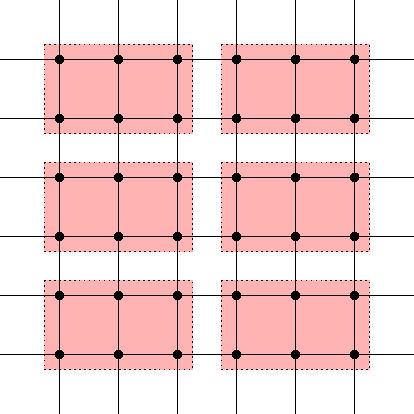
\includegraphics{Images/fig-Isingblocks.pdf}
    \caption{Pictorial idea of renormalization group (for the 2D Ising model). We course grain over the lattice by grouping the spins into blocks, then shrinking the blocks into the size of spins, and then repeating the process.}
    \label{fig-Isingblocks}
\end{figure}